% Preamble. Don't worry about it.
\documentclass{article}
\usepackage{setspace,graphicx}
\usepackage[utf8]{inputenc}
\usepackage[left=1in,top=1in,right=1in,bottom=1in]{geometry} % Document margins
\onehalfspacing

% Setting the depth for Table of Contents
\setcounter{tocdepth}{1}

\begin{document}

% --- TITLE PAGE ---
\title{Donnervögel Consulting \\ Streamlined Grading System}
\author{\textbf{Phase Lead: Ian Pun} \\ Markus Balaski \\ Stephen Laboucane \\
  Graeme Smith \\ Jordan Toering \\  Colin Woodbury \\ Chazz Young}
\date{\today}
\maketitle
\clearpage
% ------------------

% --- REVISION HISTORY ---
\textbf{Revision History}
\begin{center}
  \begin{tabular}{| c | c | c | l |}
    \hline
    Version & Date & Members & Changes\\
    \hline
    1.0 & 2014 Mar 07 (Fri) & Markus B. & Document created\\
    & & Graeme S. & \\
    & & Jordan T. & \\
    & & Stephen L. & \\
    & & Ian P. & \\
    & & Colin W. & \\
    & & Chazz Y. & \\
    \hline
  \end{tabular}
\end{center}
\clearpage
% ------------------------

% --- TABLE OF CONTENTS ---
\tableofcontents
\clearpage
% -------------------------

% ---
\section{Product Overview}  % 5 Marks
% THIS SHOULD BE 1/2 TO 1 PAGE IN LENGTH!
% Markus will do this.

% ---
\section{Getting Started}
\emph{No contents here.}

\subsection{Software Requirements}

\subsection{Hardware Requirements}

\subsection{Installation}

\subsection{Running the Application}

\subsection{UAT Installation}

% ---
\section{Functions and User Interface Description}  % 30 Marks total
% This is a very big section.
% 1. How is a function selected?
% 2. How is input entered? (Include pictures)
% 3. What keys need to be pressed?
% 4. What will the user see when a step is performed correctly?
% 5. What will the user see when a step is performed incorrectly? (errors)
\subsection{Login}

\subsection{Landing Page}
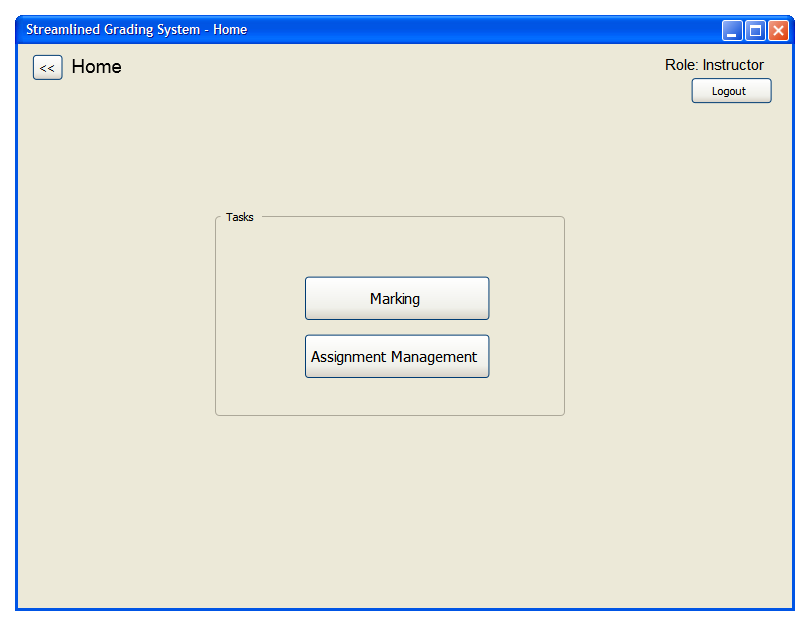
\includegraphics[scale=0.55]{../images/UIMockups/pngs/LandingPage}
The Landing Page is shown to all users of the system following login.  The Tasks
box shows actions that each user can do.  It does not show actions the user
cannot do. The above represents what an Instructor would see upon logging in.

\subsection{Manage Courses}

\subsection{Modify Courses}

\subsection{Create/Modify Activity (Detailed)}
\begin{enumerate}
  \item Log in to the system as an Instructor.
  \item The following screen will be shown.  Press the \textbf{Assignment Management} button.
  \begin{center} 
   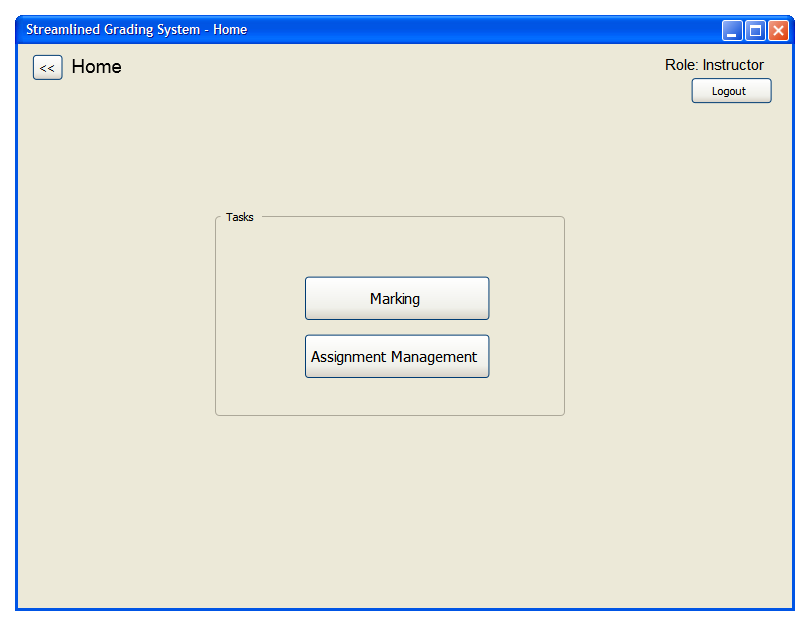
\includegraphics[scale=0.55]{../images/UIMockups/pngs/LandingPage}
  \end{center}
  \item The following screen will be shown. Select the \textbf{New Activity} button.
  \begin{center}
  NEED A SCREEN FOR THIS
  \end{center}
  \item The following screen will be shown.
   \begin{center} 
   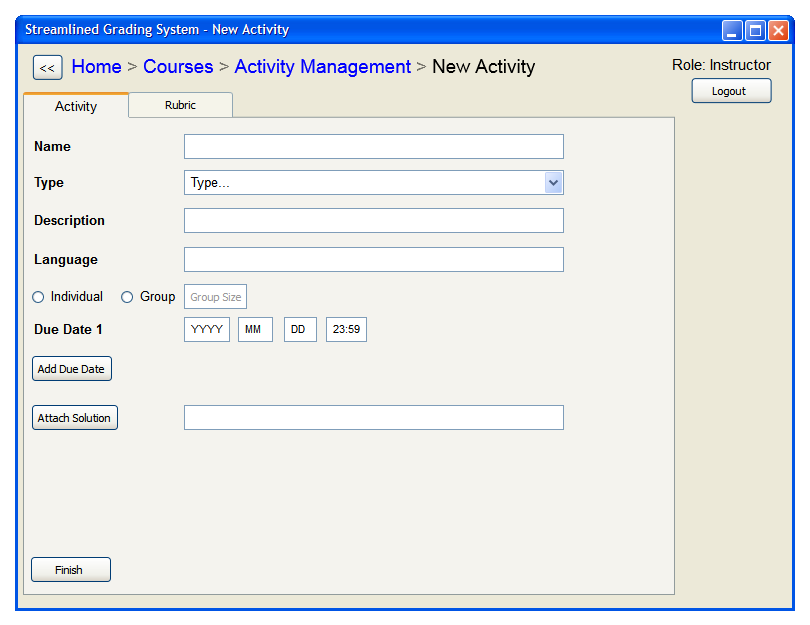
\includegraphics[scale=0.55]{../images/UIMockups/pngs/newActivity}
  \end{center}
  To create the activity, complete the following:
  \begin{enumerate}
  \item Enter a name for the activity in the \textbf{Name} text field by clicking on 
  it and typing it in.
  \item Select the type of the activity from the \textbf{Type} drop down box.
  This can be an Essay, a Problem Set, or a Programming activity.
  \item Enter a description for the activity by clicking on the \textbf{Description} 
  text field and typing it in.
  \item Enter the language of the activity by clicking on the \textbf{Language} text
  field and typing it in. This can be either a spoken language such as English 
  for an Essay or Problem Set, or a programming language such as Java for a Programming
  activity.
  \item Click on the appropriate radio to make it an \textbf{Individual} or 
  \textbf{Group} activity. If \textbf{Group} is chosen, type in the group size in the 
  adjacent field.
  \item Enter the date and time the activity is due in the \textbf{Due Date} fields 
  in the Year, Month, Day format, followed by the time it is due on that due in the 24-hour 
  format. The default time is 23:59.
  \item A solution can be attached by clicking the \textbf{Attach Solution} button and 
  selecting the desired file from the Explorer window. Alternatively, the path can be 
  typed directly into the adjacent field.
  \end{enumerate}
  \item The following is how the New Activity screen could look with some additional options. 
  \begin{center} 
   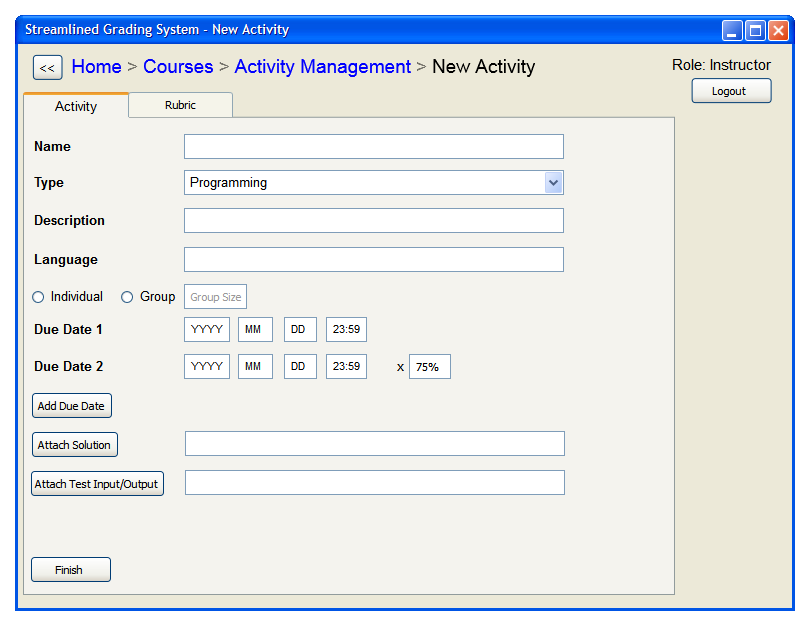
\includegraphics[scale=0.55]{../images/UIMockups/pngs/newActivityDetailed}
  \end{center}
  \begin{enumerate}
  \item Clicking \textbf{Add Due Date} adds new fields to add an additional date that can 
  be before or after the original due date. The new date can be entered in the same manner 
  as as above. The extra field is the multiplier for penalties/bonuses. For example, 
  entering "75" is equivalent to a 25\% penalty, and entering "110" would be equivalent 
  to a 10\% bonus.
  \item The option \textbf{Attach Test Input/Output} becomes available if \textbf{Type} 
  is set to \textbf{Programming}. This functions exactly as \textbf{Attach Solution}.
 \end{enumerate}
 \item To work on the rubric for the activity, click on the \textbf{Rubric} tab at the 
 top of the page that is underneath the breadcrumbs. This will open the rubric tab and 
 show the following screen.
 \begin{center} 
   NEED AN IMAGE FOR THIS
   \\ THEN THIS STEP NEEDS TO BE COMPLETED
 \end{center}
 \item Once all the desired information about the activity has been entered in correctly, 
 clicking \textbf{Finish} will create the activity and open the \textbf{Activity Management} 
 page.
  \begin{center} 
   PUT THE ACTIVITY MANAGEMENT IMAGE HERE
 \end{center}
\end{enumerate}
\textbf{*NOTE: }If the user tries to navigate away or clicks \textbf{Logout} when 
there are unsubmitted changes, a prompt will be shown asking the user to confirm that 
they intend to navigate away from the current page without saving. (As shown below)
 \begin{center} 
   WARNING SCREEN HERE
 \end{center}


\subsection{Modify Activity}

\subsection{Copy Activity}

\subsection{Activity Marking (Detailed)}
\begin{enumerate}
  \item Log in to the system as a user who has marking privileges.
  \item The following screen will be shown.  Press the \textbf{Marking} button.
  \begin{center} 
   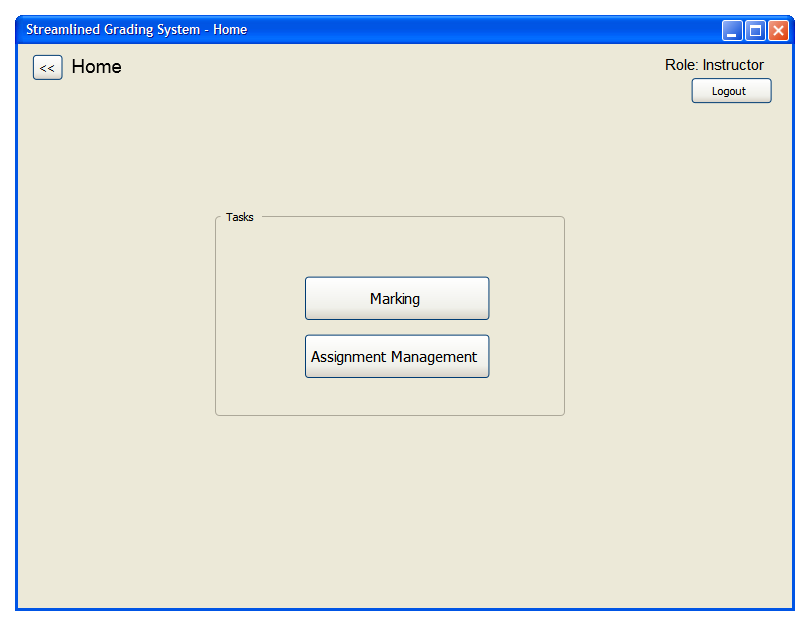
\includegraphics[scale=0.55]{../images/UIMockups/pngs/LandingPage}
  \end{center}
  \item The following screen will be shown.  Select the course that you wish
    to do marking for from the drop-down list, then press \textbf{Ok}.
    \begin{center} 
      STEPHEN'S COURSE SELECTION IMAGE HERE
    \end{center}
  \item The following screen will be shown.  Students are listed down the left
    side. Available activities are listed along the top.  Find the student you
    wish to mark for, and select the corresponding activity, then press \textbf{Ok}.
  \begin{center} 
    STEPHEN'S STUDENT/ACTIVITY MATRIX IMAGE HERE
  \end{center}
  \item The assignment's marking screen will be shown.  The marking screen
    displays the rubric, sample solution, and the student's submission.
  \begin{center} 
   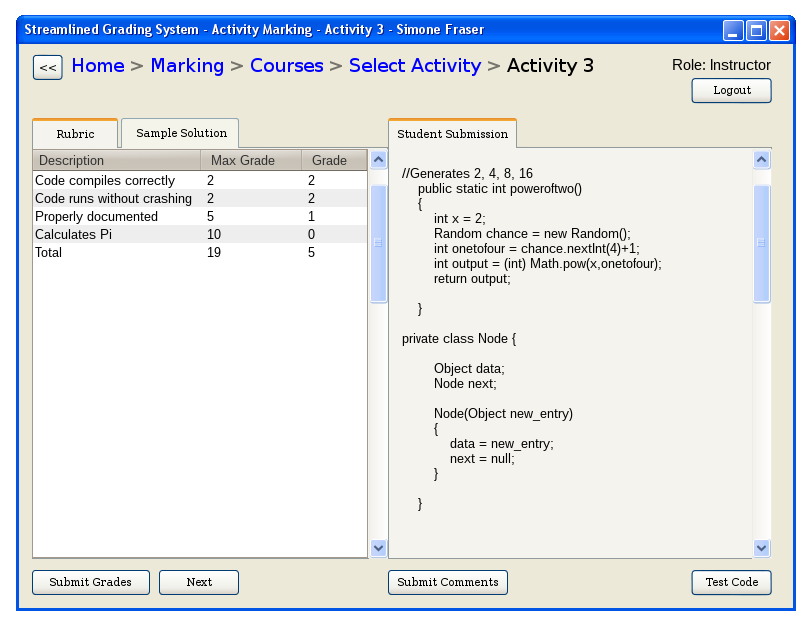
\includegraphics[scale=0.55]{../images/UIMockups/pngs/activityMarking}
  \end{center}
    Perform the grading process as follows:
    \begin{enumerate}
      \item Perform necessary analysis on the student's work. 
      \item Read rubric points and enter a number into the available box 
        based on your analysis of the student's work.
      \item Repeat step (a) for remaining rubric points.
      \item A total will be shown at the bottom of the rubric to reflect the
        student's final grade on the activity.
       \item Click the \textbf{Submit} button to update the marks database with
         the changes made.
    \end{enumerate}

  \item If desired: Press the \textbf{Submit} button to move to the next
    student's submission of the same activity.
\end{enumerate}
\textbf{*NOTE: }If the user clicks \textbf{Back}, \textbf{Next}, \textbf{Logout}
or \textbf{Anywhere in the Breadcrumb} when there are unsubmitted changes, a
prompt will be shown asking the user to confirm that they intend to navigate away
from the current page without saving. (As shown below)

\begin{center}
  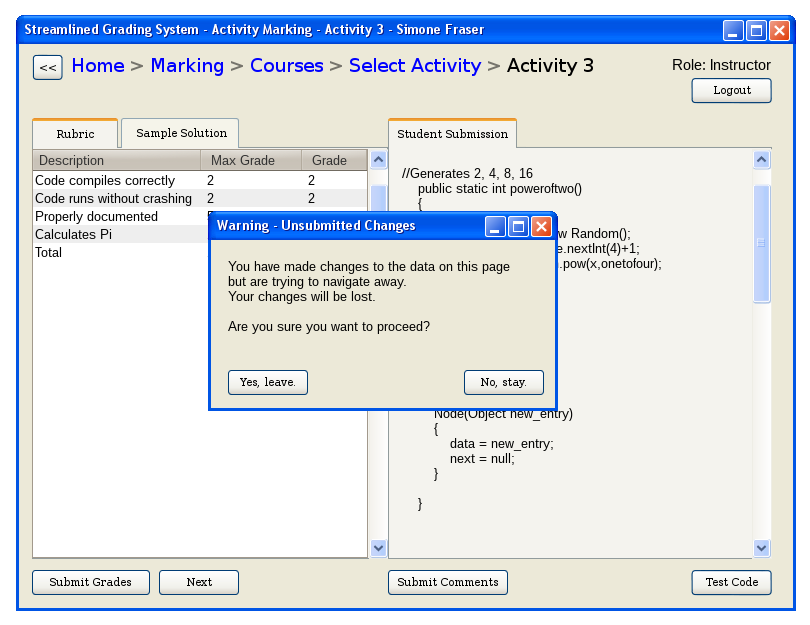
\includegraphics[scale=0.55]{../images/UIMockups/pngs/activityMarkingWarning}
\end{center}

\subsection{Test Suite}
\begin{center}
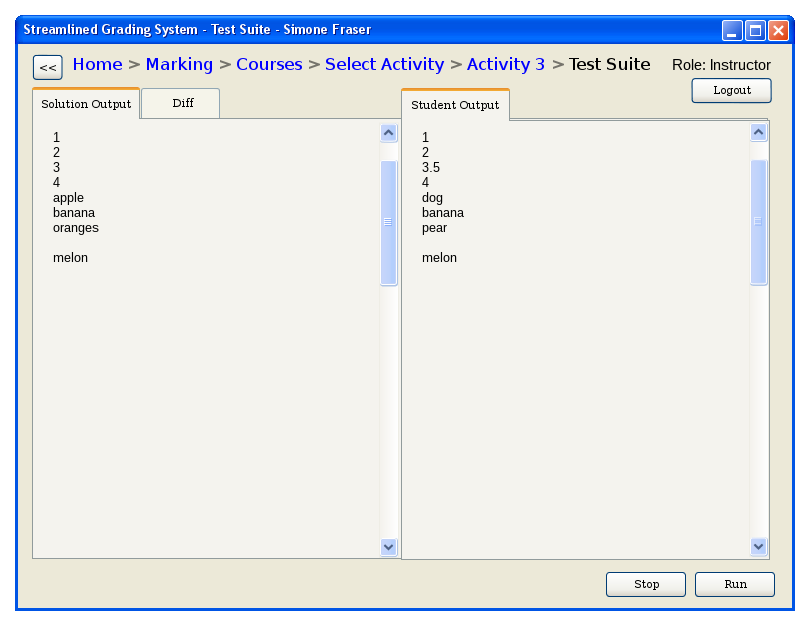
\includegraphics[scale=0.55]{../images/UIMockups/pngs/SRS_TestSuite_Split}
\end{center}
The Test Suite shows the \textbf{Solution Output}, the \textbf{Student Output},
and the \textbf{Diff}.
The three windows can be docked together (tabbed) or positioned that each
window takes up $\frac{1}{3}$ of the screen space.
The \textbf{Diff} window intelligently shows the difference between
solution and submitted code.

\subsection{Manage Database}
+%INSERT "databaseManagement" PAGE HERE%
The user will be led to a page with two options: \textbf{Backup Database} and
\textbf{Restore Database}
\begin{itemize}
  \item Backup Database
    By clicking this, the system will create a backup of the entire system.
    It will be suffixed with the data of backup. A confirmation message will
    appear when completed.
  \item Restore Database
    By clicking this, the user will be given a pop-up to select the backup to
    restore the database to (organized from newest to oldest). It will then
    prompt a second time to confirm the restoration of the system to that backup.

%INSERT SELECT BACKUP HERE%
\end{itemize}
\subsection{Manage User Accounts}
%INSERT accountCreationModification FORM HERE%
A form will appear on clicking this. 
If the user wishes to modify an existing account: \\
the user must check the \textbf{Modify} check-box. The grayed out drop down menu and
save button will become active, and the \textbf{Create} button will be grayed out.
The user will select the account to edit (organized alphabetically by username).
Upon selecting a user, the form fields will populate and become editable. After
the user has finished editing the fields, the user must click \textbf{Save}. The system
will save the changes and return to the Landing page. \\
\textbf{*NOTE*} If the user wishes to generate a new password, a confirmation
prompt will appear asking for confirmation.\\
If the user wishes to create a new account: \\
The user must not check the \textbf{Modify} box. By doing so, the \textbf{Save}
button and the drop-down menu for selecting an account will be grayed out.
The user then fills the form as normal. After the user has finished, the user
must click \textbf{Save}.
\subsection{Manage System Logs}
%INSERT SYSTEM LOG SELECT HERE%
Upon clicking this button, the user will be prompted with a drop-down menu of
the system logs (organized chronologically, with the default being the log
from the current day). The system will then display the log activity for
that day.

% ---
\section{Quick Reference}  % 9 Marks

% ---
\section{Known Bugs}
There are no bugs, our software is perfect.

\end{document}
